\chapter{Results and Evaluation\label{chap:evaluation}}
% Around 9-10 pages
% Do I need to add experimental Design stuff here?
\section{Quantitative Outlook with the Metrics}
As previously outlined, the plots are colored to easily distinguish the counterfactuals from AIDE (green), DiCE (blue), and DiCE-genetic/GeCo (red). These charts are best viewed in the browser as \inlinecode{plotly} provides them as interactive HTML files and they can be filtered by explainer method in the case of overlaps.


\begin{figure}[!htbp]
    \centering
    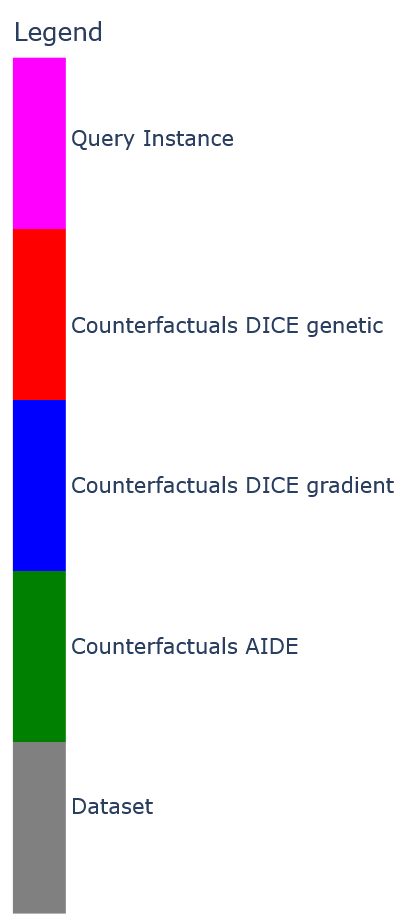
\includegraphics[angle=90, width=\textwidth]{images/legend.png}
    \caption{Image of the legend for the metric and parallel coordinates plots.}
    \label{fig:legend-plots}
\end{figure}
\begin{figure}[!htbp]
    \centering
    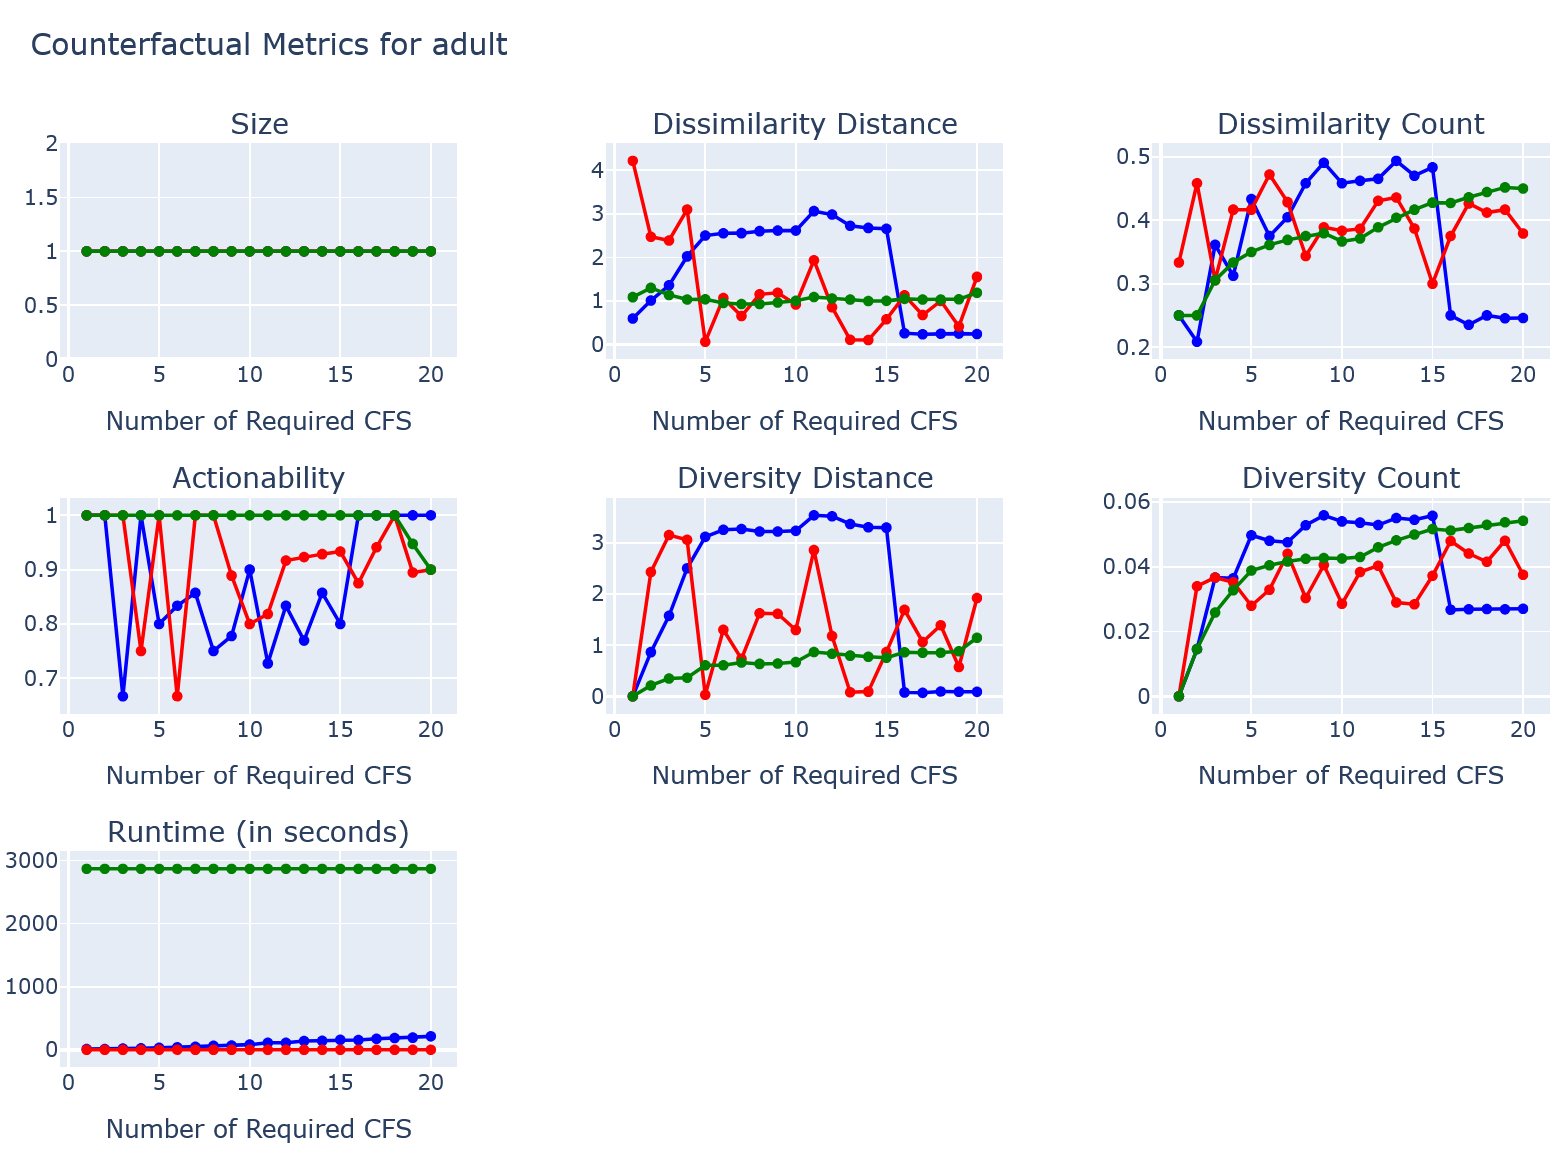
\includegraphics[width=\textwidth]{images/metrics-adult.png}
    \caption{Image of the metrics for the explainers on the adult dataset, varying the required number of
required counterfactuals.}
    \label{fig:metrics-adult}
\end{figure}
\begin{figure}[!htbp]
    \centering
    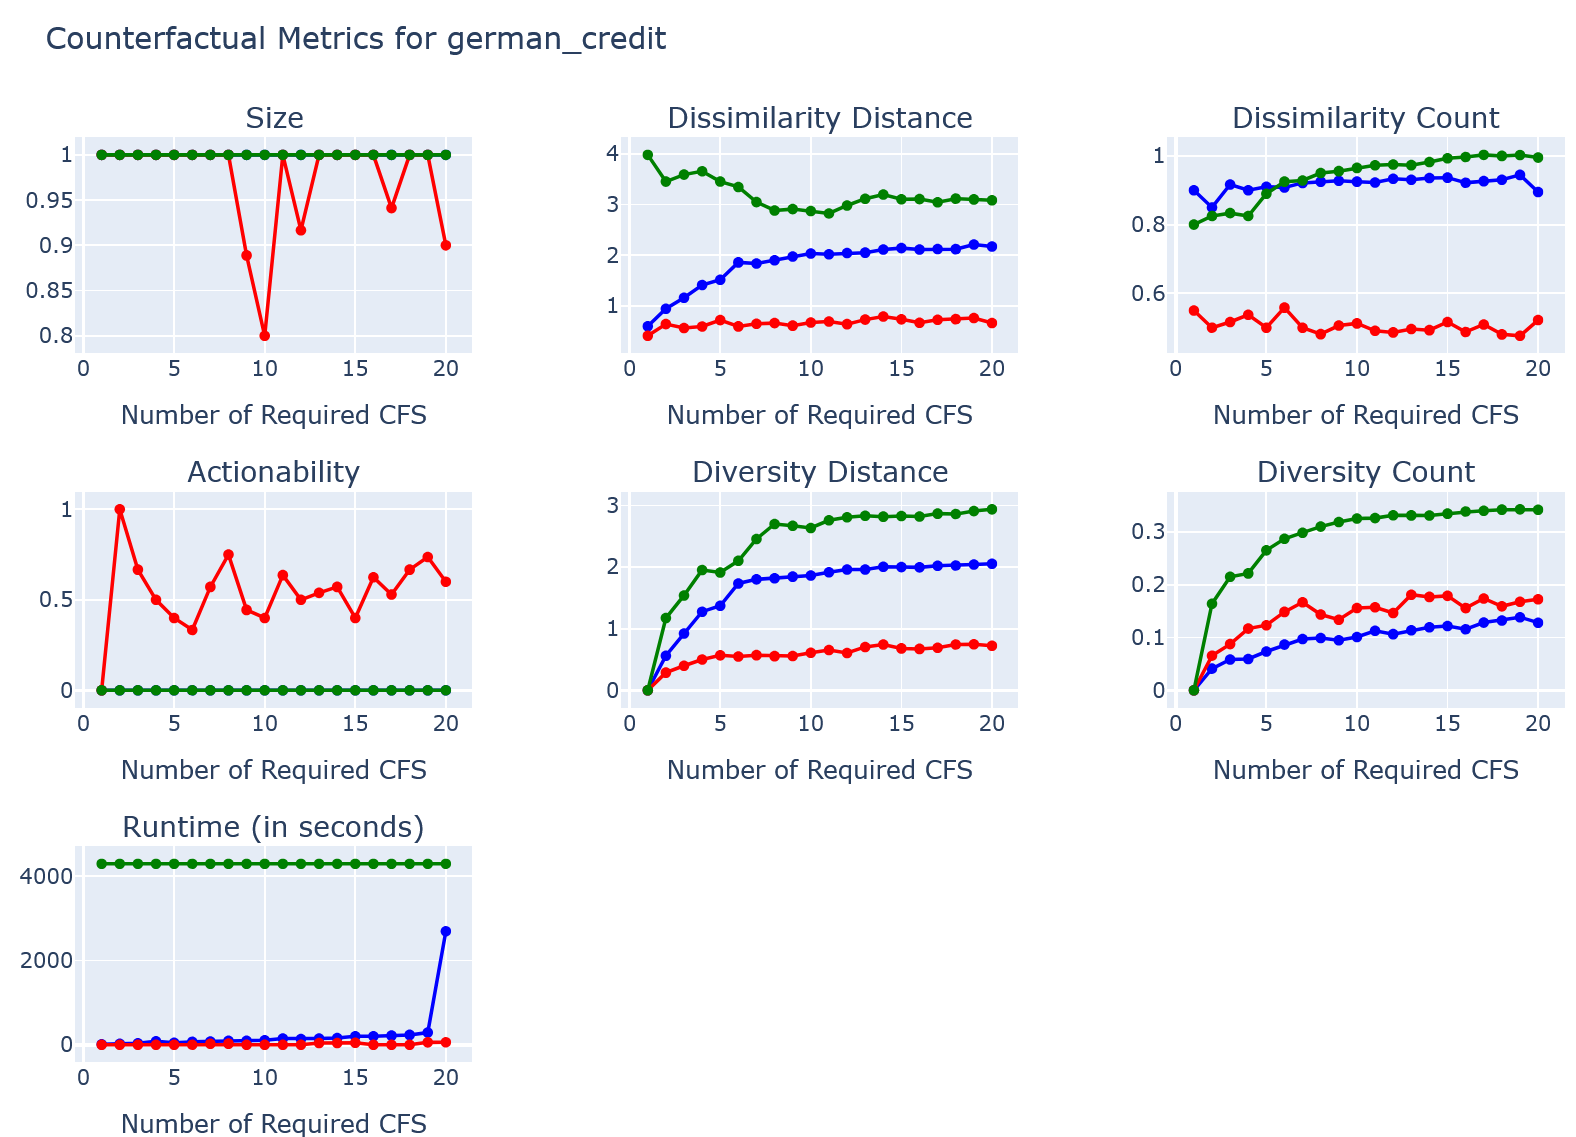
\includegraphics[width=\textwidth]{images/metrics-german_credit.png}
    \caption{Image of the metrics for the explainers on the german\_credit dataset, varying the required number of
required counterfactuals.}
    \label{fig:metrics-german_credit}
\end{figure}
\begin{figure}[!htbp]
    \centering
    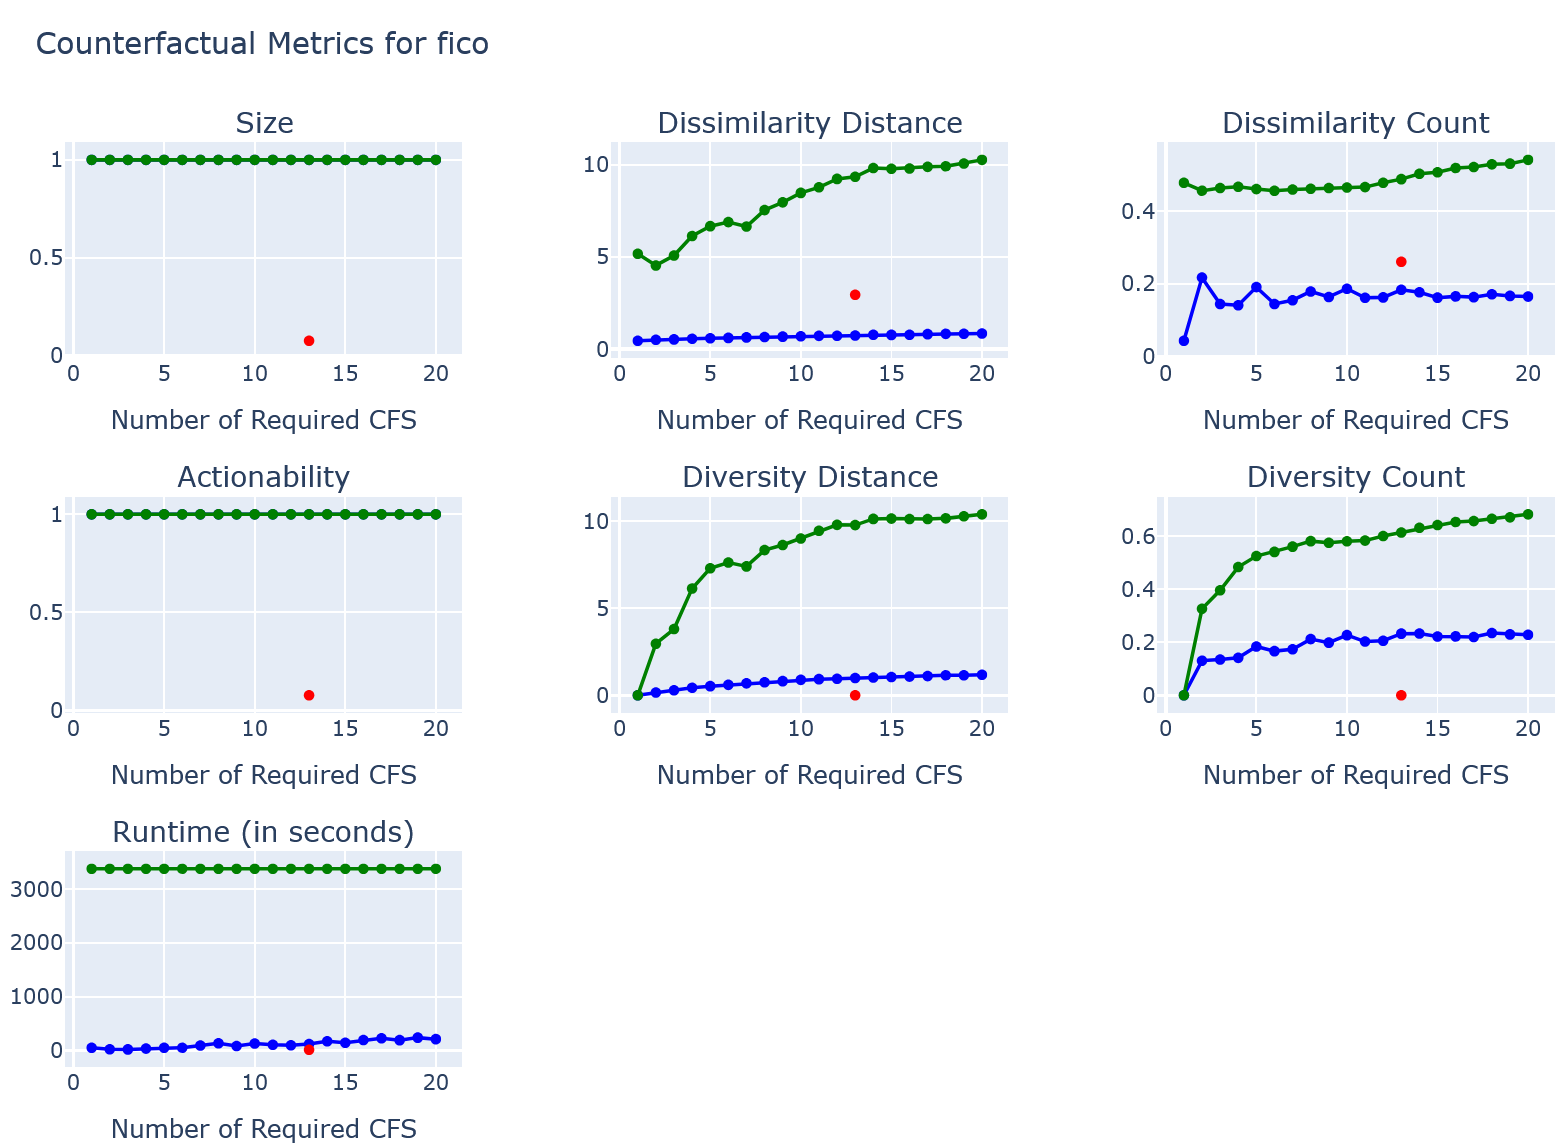
\includegraphics[width=\textwidth]{images/metrics-fico.png}
    \caption{Image of the metrics for the explainers on the fico dataset, varying the required number of
required counterfactuals.}
    \label{fig:metrics-fico}
\end{figure}
\begin{figure}[!htbp]
    \centering
    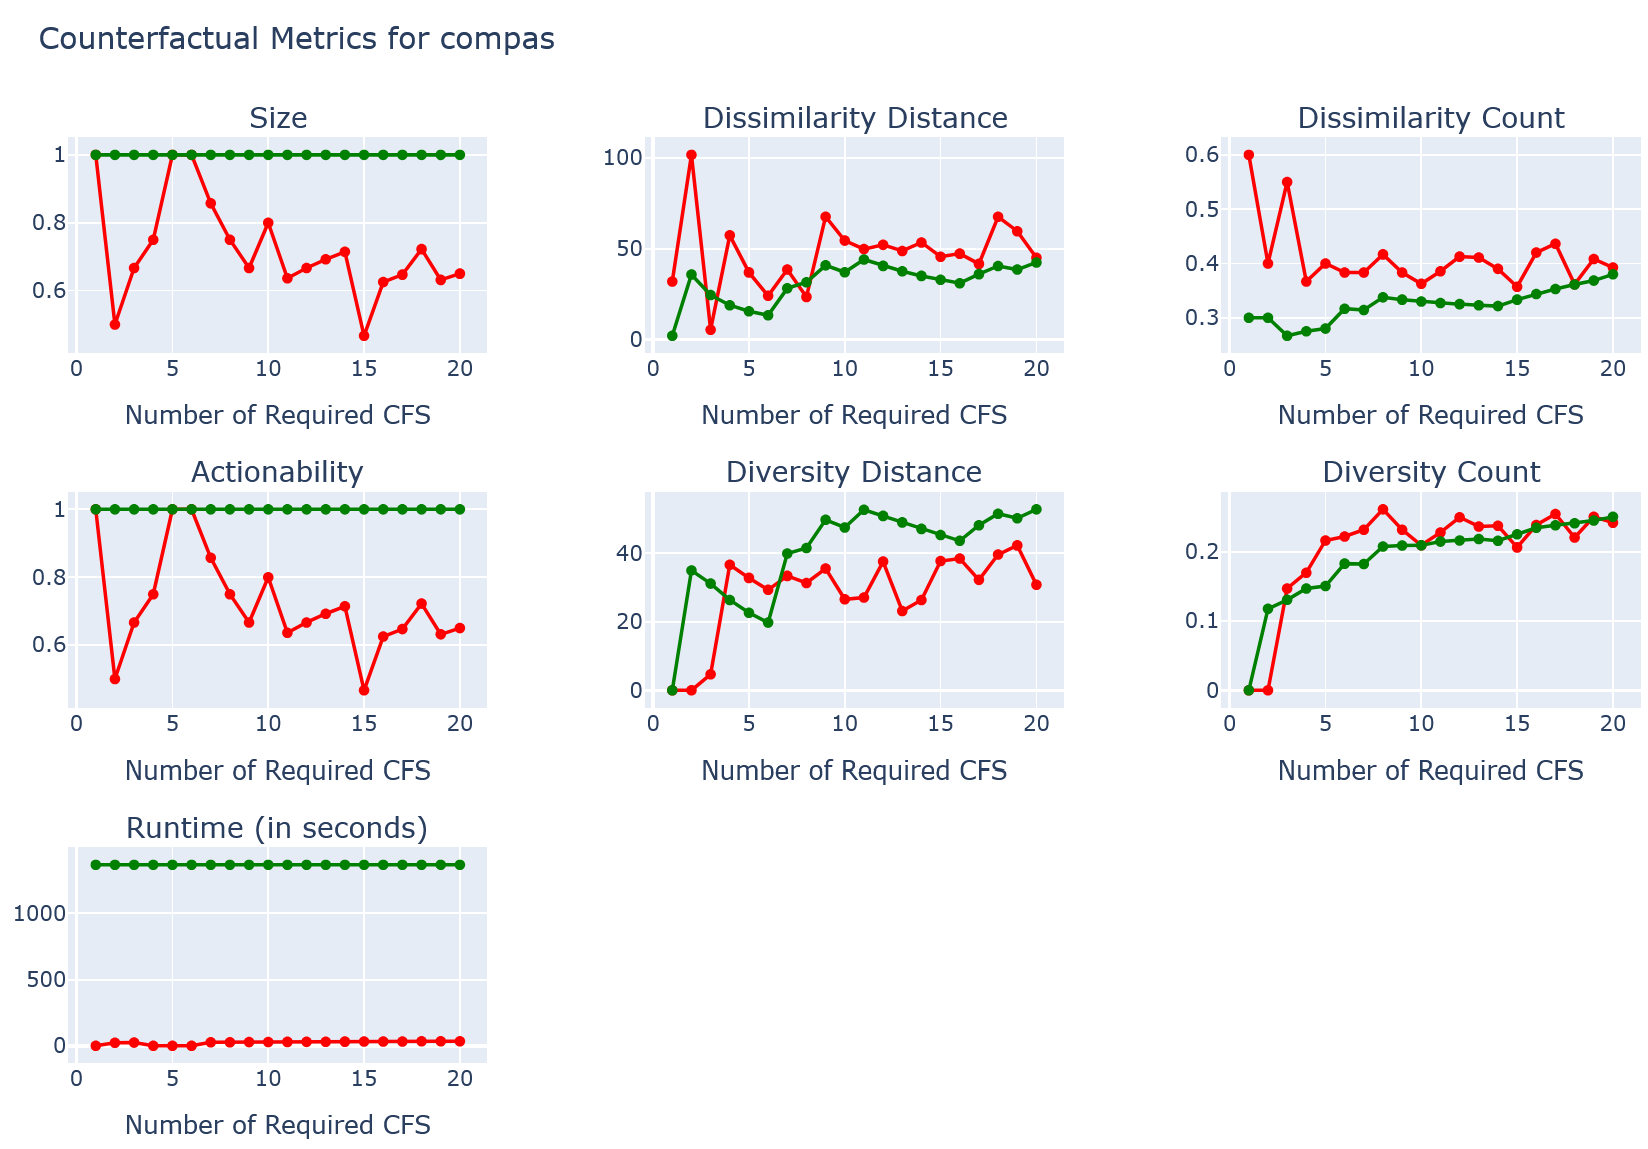
\includegraphics[width=\textwidth]{images/metrics-compas.png}
    \caption{Image of the metrics for the explainers on the compas dataset, varying the required number of
required counterfactuals.}
    \label{fig:metrics-compas}
\end{figure}

Let us examine each metric (left to right) to observe trends. For some certainty, it can be observed that the shape of the adult curves are similar to the ones in \citet{guidotti2024counterfactual} but more sharp. This makes sense, since the literature review averages the plots over all of the datasets. From the size plot, we notice that only DiCE-genetic fails to always return the required amount. Looking deeper into the algorithm this is clear since the genetic algorithm attempts to generate the specified number of CFs, but success depends on finding valid CFs that meet the desired outcome. If insufficient valid CFs are found within the iteration limit \inlinecode{maxiterations=5}, the result will contain fewer CFs. AIDE would likely have suffered from the same issue if the limit was not increased to 100. The constant size of 1 for AIDE is expected with the single-shot strategy and this is also a breeze for DiCE.

As for Dissimilarity, the count which accounts for feature level-sparsity does not seem to have large magnitudes of difference between the methods. However, it does seem that AIDE is worse, especially for when the number of required CFs is greater than 5. The Distances vary more greatly, other than fico it seems that AIDE is a lot more constant, DiCE-genetic jumps quite sharply, and DiCE rises constantly. DiCE also falls dramatically number of required CFs is greater than 15 for Adult. 

From the Actionability plot it can be observed that only AIDE return a large fraction of actionable CFs. There is some strange behavior in german\_credit where both DiCE and AIDE miserably fail. This is likely because of the amount of non-actionable columns and the long and complex column names after encoding. As \citet{guidotti2024counterfactual} points out this is expected since DiCE and it's genetic variant allow specifying the actionable features, but this check is not enforced for Validity or Actionability. On the other hand, AIDE attempts to mutate values in the set of actionable features. This is especially strange for the genetic variant since it was expected that GeCo's PLAF constraints to work it's magic, but it could that the package does not use the constraints. 

Diversity also seems to have a clear winner for counts and distance, which is AIDE. Interestingly, even though DiCE-genetic has a higher Dissimilarity distance than AIDE, AIDE has higher Diversity distance across all datasets. This shows that AIDE attempts to balance the trade-off in Diversity and Similarity. Yet again, DiCE's Diversity falls dramatically number of required CFs is greater than 15 for Adult, which is expected since of the known trade-off between Diversity and Similarity. 

Lastly, for Runtime it can be clearly seen that the $\Delta$-representation and partial evaluation in DiCE-genetic are optimizing the runtimes well. DiCE takes slightly longer to run but AIDE does take a much longer time to run. This is due to the increase in iteration limit by 10 times and due to the single-shot approach taken to generate the counterfactuals. 

\subsection{Statistical Tests}
After looking at the plots, let us employ statistical evaluation of the metrics. Since advantageous properties could be high (Diversity) or low (Dissimilarity), a One-way ANOVA (ANalysis Of VAriance) with post-hoc Tukey HSD (Honestly Significant Difference) is computed for each metric across all of the datasets. This was also computed per dataset and is available in the repository. This is done since we have three groups.
%[Should I add other precond].

\begin{table}[!htbp]
    \centering
    \centering
    \begin{tabular}{l l r r r r l}
        \toprule
        Group 1 & Group 2 & Mean Diff & p-adj & Lower & Upper & Reject \\
        \midrule
        AIDE & DiCE-genetic   & -0.1153 & 0.0 & -0.1564 & -0.0742 & True \\
        AIDE & DiCE  &  0.0000 & 1.0 & -0.0413 &  0.0413 & False \\
        DiCE-genetic & DiCE  &  0.1153 & 0.0 &  0.0713 &  0.1593 & True \\
        \bottomrule
    \end{tabular}
    \caption{Table of Tukey's HSD Test results for Size (ANOVA p-value = \SI{4.492443e-11}{})}
    \label{tab:tukey-results-size}
\end{table}

\begin{table}[!htbp]
    \centering
    \begin{tabular}{llrrrrl}
        \toprule
        Group 1 & Group 2 & Mean Diff & p-adj & Lower & Upper & Reject \\
        \midrule
        AIDE          & DiCE-genetic   &  5.3934  & 0.1207 &  -1.05   & 11.8369  & False \\
        AIDE          & DiCE  & -9.5077  & 0.0019 & -15.9815 &  -3.0338 & True  \\
        DiCE-genetic & DiCE  & -14.9011 & 0.0    & -21.7936 &  -8.0087 & True  \\
        \bottomrule
    \end{tabular}
    \caption{Table of Tukey's HSD Test results for Dissimilarity Distance (ANOVA p-value = \SI{3e-6}{})}
    \label{tab:tukey-results-dis-dist}
\end{table}

\begin{table}[!htbp]
    \centering
    \begin{tabular}{llrrrrl}
        \toprule
        Group 1 & Group 2 & Mean Diff & p-adj & Lower & Upper & Reject \\
        \midrule
        AIDE          & DiCE-genetic   & -0.0976 & 0.0479 & -0.1944 & -0.0007 & True  \\
        AIDE          & DiCE  & -0.0492 & 0.4582 & -0.1465 &  0.0481 & False \\
        DiCE-genetic & DiCE  &  0.0484 & 0.5139 & -0.0553 &  0.1520 & False \\
        \bottomrule
    \end{tabular}
    \caption{Table of Tukey's HSD Test results for Dissimilarity Count (ANOVA p-value = \SI{6.0451e-2}{})}
    \label{tab:tukey-results-dis-count}
\end{table}
\begin{table}[!htbp]
    \centering
    \begin{tabular}{llrrrrl}
        \toprule
        Group 1 & Group 2 & Mean Diff & p-adj & Lower & Upper & Reject \\
        \midrule
        AIDE          & DiCE-genetic   & -0.0329 & 0.8734 & -0.1897 & 0.1238 & False \\
        AIDE          & DiCE  & -0.1219 & 0.1633 & -0.2794 & 0.0356 & False \\
        DiCE-genetic & DiCE  & -0.0890 & 0.4235 & -0.2567 & 0.0787 & False \\
        \bottomrule
    \end{tabular}
    \caption{Table of Tukey's HSD Test results for Actionability (ANOVA p-value = \SI{0.181364}{})}
    \label{tab:tukey-results-act}
\end{table}

\begin{table}[!htbp]
    \centering
    \begin{tabular}{llrrrrl}
        \toprule
        Group 1 & Group 2 & Mean Diff & p-adj & Lower & Upper & Reject \\
        \midrule
        AIDE          & DiCE-genetic   &  -2.9441 & 0.4211 &  -8.4737 &   2.5856 & False \\
        AIDE          & DiCE  & -11.3308 & 0.0    & -16.8865 &  -5.7751 & True  \\
        DiCE-genetic & DiCE  &  -8.3867 & 0.0028 & -14.3016 &  -2.4718 & True  \\
        \bottomrule
    \end{tabular}
    \caption{Table of Tukey's HSD Test results Diversity Distance (ANOVA p-value = \SI{1.2e-5}{})}
    \label{tab:tukey-results-div-dist}
\end{table}

\begin{table}[!htbp]
    \centering
    \begin{tabular}{llrrrrl}
        \toprule
        Group 1 & Group 2 & Mean Diff & p-adj & Lower & Upper & Reject \\
        \midrule
        AIDE          & DiCE-genetic   & -0.1434 & 0.0    & -0.2017 & -0.0851 & True  \\
        AIDE          & DiCE  & -0.1587 & 0.0    & -0.2173 & -0.1001 & True  \\
        DiCE-genetic & DiCE  & -0.0153 & 0.8322 & -0.0776 &  0.0471 & False \\
        \bottomrule
    \end{tabular}
    \caption{Table of Tukey's HSD Test results for Diversity Count (ANOVA p-value = \SI{8.018792e-11}{})}
    \label{tab:tukey_results}
\end{table}
\begin{table}[!htbp]
    \centering
    \begin{tabular}{llrrrrl}
        \toprule
        Group 1 & Group 2 & Mean Diff & p-adj & Lower & Upper & Reject \\
        \midrule
        AIDE          & DiCE-genetic   & -2963.6502 & 0.0   & -3244.5292 & -2682.7712 & True \\
        AIDE          & DiCE  & -2819.7193 & 0.0   & -3101.9232 & -2537.5154 & True \\
        DiCE-genetic & DiCE  &   143.9309 & 0.496 &  -156.5187 &   444.3806 & False \\
        \bottomrule
    \end{tabular}
    \caption{Table of Tukey's HSD Test results for Runtime (ANOVA p-value = \SI{2.700452e-71}{})}
    \label{tab:tukey_results}
\end{table}


So to put it into text here is what was found:
\begin{itemize}
    \item \textbf{Size:} This is a tie between AIDE and DiCE. Both achieve perfect scores (1.0), while DICE-genetic is significantly worse. 
    \item \textbf{Dissimilarity Distance:} DiCE is the best performer with the lowest mean (1.43, AIDE: 10.94, DiCE-genetic: 16.33) with significant differences from others.
    \item \textbf{Dissimilarity Count:} DiCE-genetic only marginally significantly overcomes the other explainers (ANOVA p=0.06).
    \item \textbf{Actionability:} Although not statistically significant (ANOVA p=0.18), AIDE is the best here. if not for the unexpected behavior in german\_credit it would most likely been significant.
    \item \textbf{Diversity Distance:} AIDE is the most diverse (12.84, DiCE:1.54, DICE-genetic: 9.90). However, it does not significantly triumph over DiCE-genetic.
    \item \textbf{Diversity Count:} AIDE significantly prevails over both. But there is not a significant difference between the other explainers.
    \item \textbf{Runtime:} Despite DICE-genetic being faster than AIDE, it is not significantly faster than DiCE (Tukey HSD p=0.496).
\end{itemize}

Consequently for both of the research questions (\textbf{RQ1} and \textbf{RQ2}), even though AIDE performed well for the four out of the seven metrics it is not hands down better for generating counterfactuals than DiCE or genetic-DiCE. In order to dig deeper, the parallel coordinate plots will need to be looked at.

% Two parts to digging deep 
%Make conclusions about research question and open up new ones and go into Parallel Coordinate Plots. 
\section{Qualitative Outlook with the Parallel Coordinates Plots}
In the parallel coordinates plots, the dataset (gray), the query instance (magenta) are added. These counterfactuals are plotted for when the required number is 20. It is stressed that the charts are particularly better experienced on the browser. These plots are richly interactive. The lines can be dragged along the axes to filter regions and the axis can be dragged names across the plot to rearrange variables. This is useful for the target class. Another suggestion, is to view the german\_credit and fico plots on a wider display since the columns names are long and can be hard to distinguish in the plots.

\begin{figure}[!htbp]
    \centering
    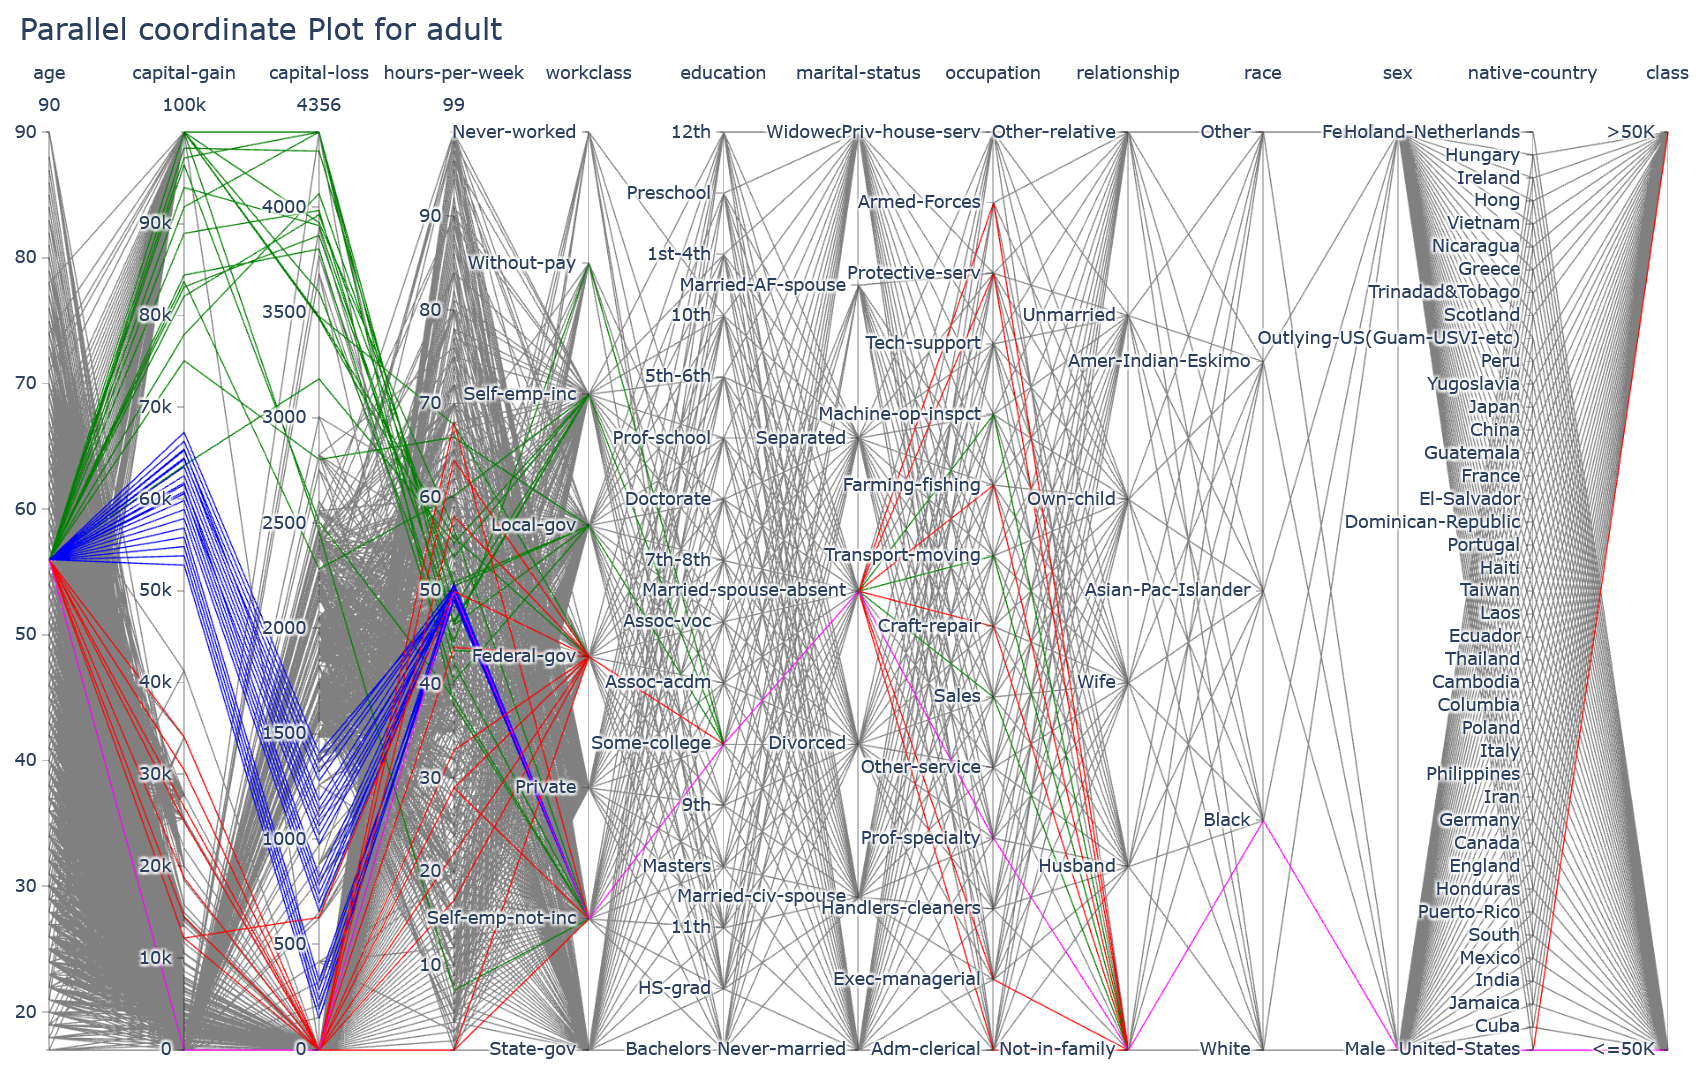
\includegraphics[width=\textwidth]{images/pcp-adult.png}
    \caption{Parallel coordinate plot for the explainers on the adult dataset.}
    \label{fig:pcp-adult}
\end{figure}

Due to space constraints, only the adult dataset will be analyzed thoroughly axis-by-axis. The actionability is pretty high across all explainers so the non-actionable columns (age, education, marital status, relationship, race, sex, native country) will be ignored. These will appear as if they are merging into the original query instance in the plot. For capital-gain, it can be seen that DiCE's CFs are in a range that the dataset is not and the deltas between each CFs are very similar. This is likely due to the "repulsions" from the \verb|dpp_diversity| term. On the other hand, AIDE and DiCE-genetic are on opposite sides of this spectrum. With AIDE selecting the higher-end while, DiCE-genetic opting for options closer to the query instance. 

A similar story can be seen with capital-loss, DiCE's CFs are again in a range of low concentration compared to the rest of the dataset. DiCE-genetic hurts itself here in terms of diversity since the capital-loss here is the same for all CFs (0). Likewise, AIDE's CFs are near the upper end of capital-loss.

hours-per-week experiences a different behavior compared to the above two axes. It's hard to gauge the deltas of DiCE but the values seems to concentrated around the query instances values (50). DiCE-genetic's values seem to jump around a lot here. This is likely why the  Dissimilarity is high. AIDE's values also jump around quite a bit but has clusters closer to the query instance due immune-network approach that tries to maintain multiple local optima.

For our first categorical feature, workclass, DiCE really struggles here not changing this variable for any counterfactual. DiCE-genetic does not perform much better only suggesting one other category... Federal-gov. These methods do this even though if the target is filtered there are a significant number of instances across six of the categories. AIDE does shine here but one CF does oddly suggest Without-pay where no other data point has a salary greater than 50k with that category.

Lastly, the other categorical feature, occupation, DiCE experiences the same issues. However, DiCE-genetic does significantly improve here maintaining many categories. AIDE still performs well here.

\begin{figure}[!htbp]
    \centering
    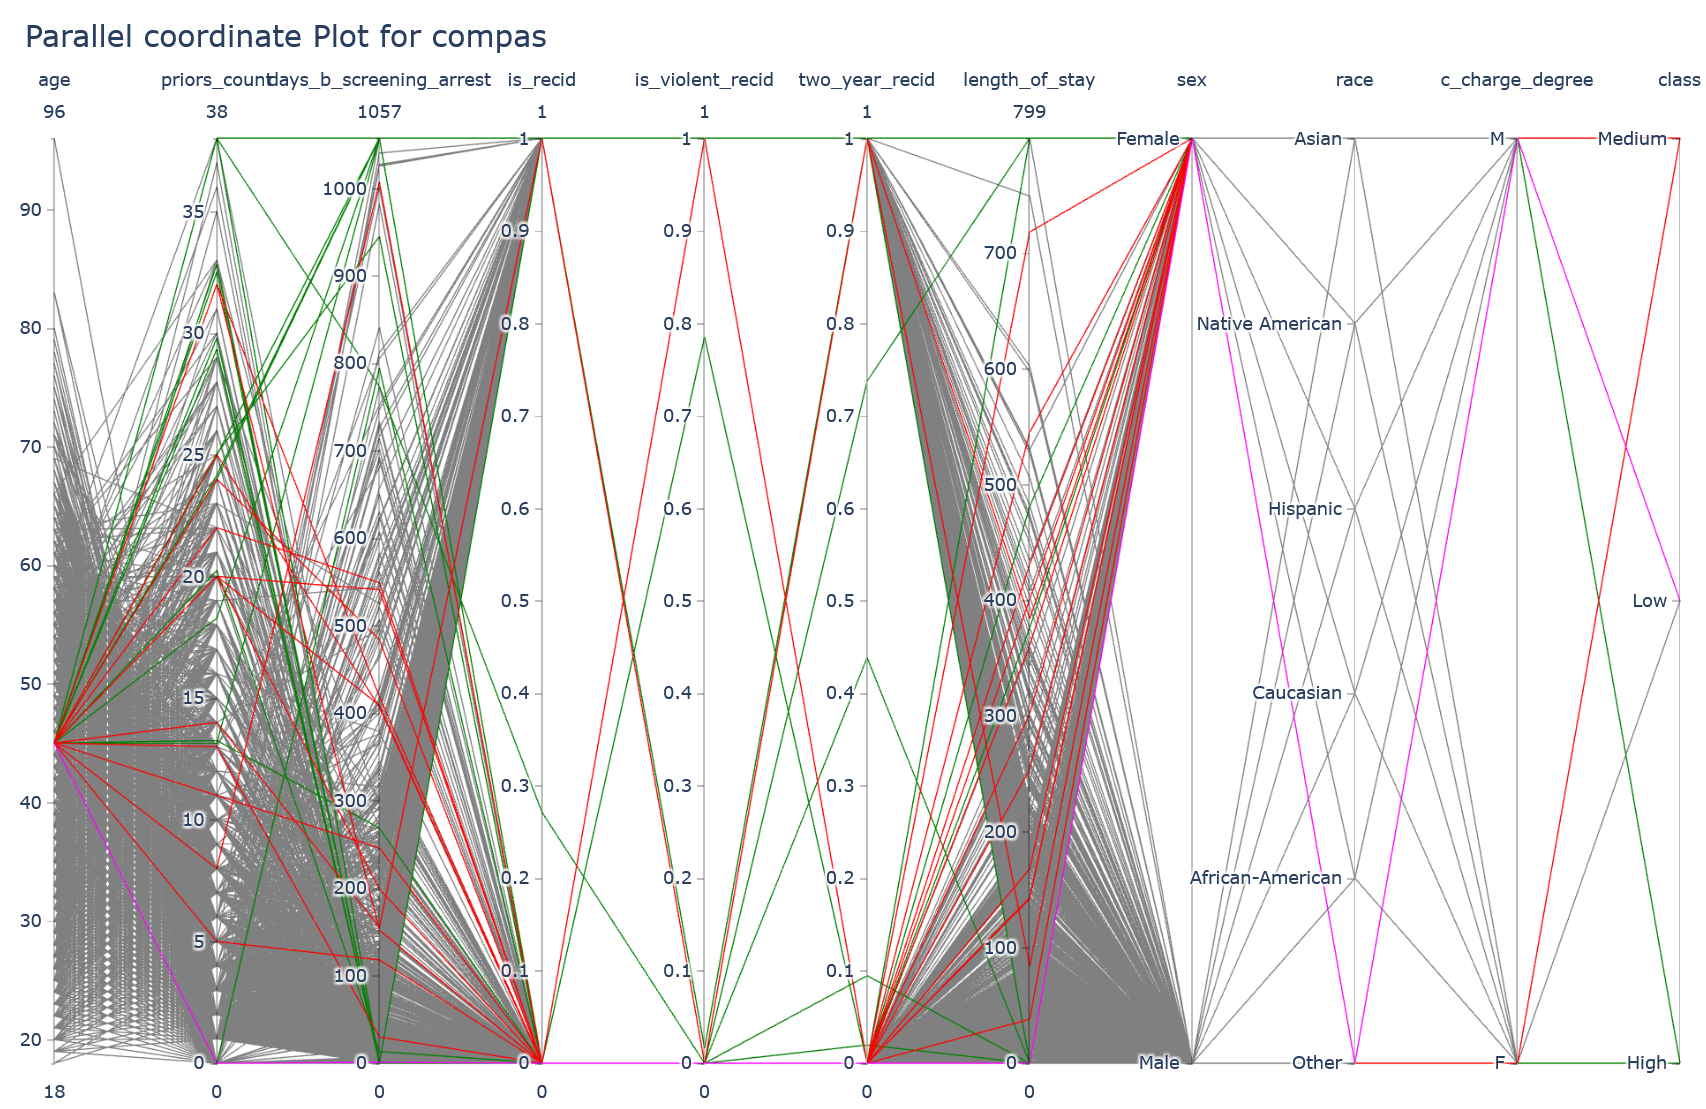
\includegraphics[width=\textwidth]{images/pcp-compas.png}
    \caption{Image of parallel coordinates plot for the explainers on the compas dataset.}
    \label{fig:pcp-compas}
\end{figure}
\begin{figure}[!htbp]
    \centering
    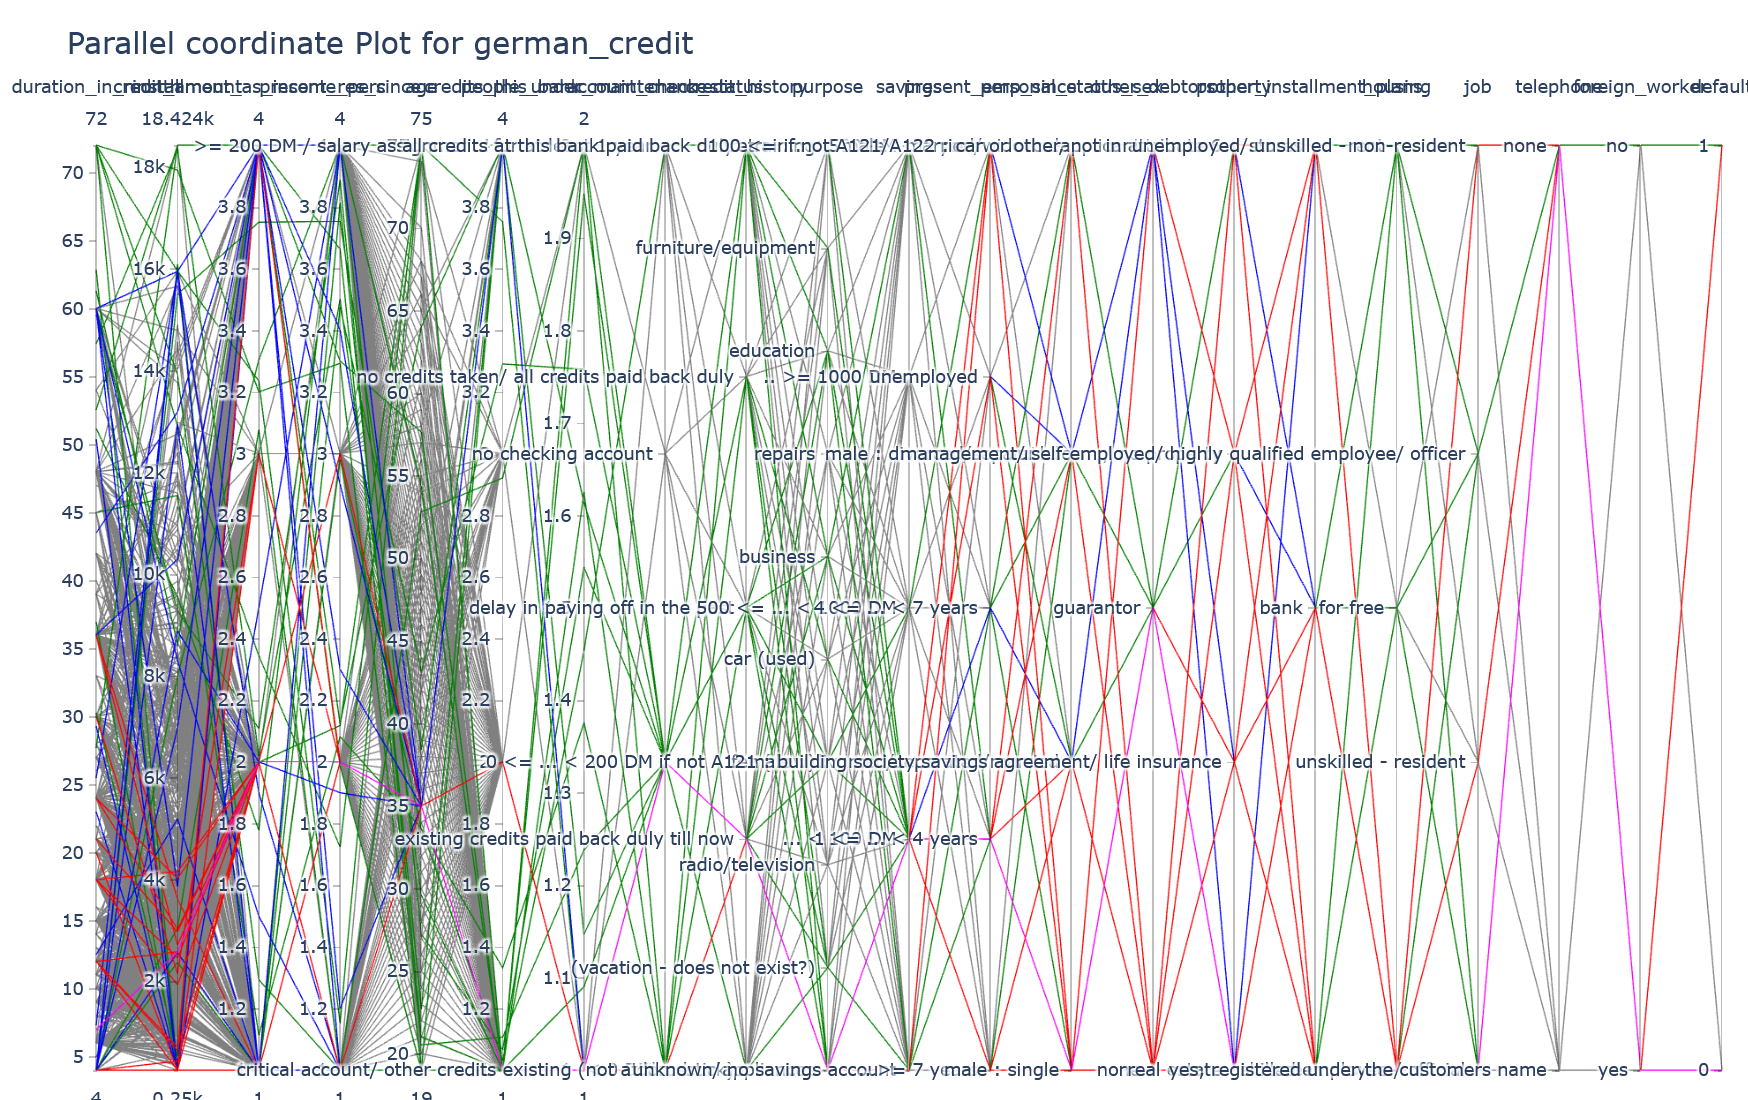
\includegraphics[width=\textwidth]{images/pcp-german_credit.png}
    \caption{Image of the parallel coordinates plot for the explainers on the german\_credit dataset.}
    \label{fig:pcp-german_credit}
\end{figure}
\begin{figure}[!htbp]
    \centering
    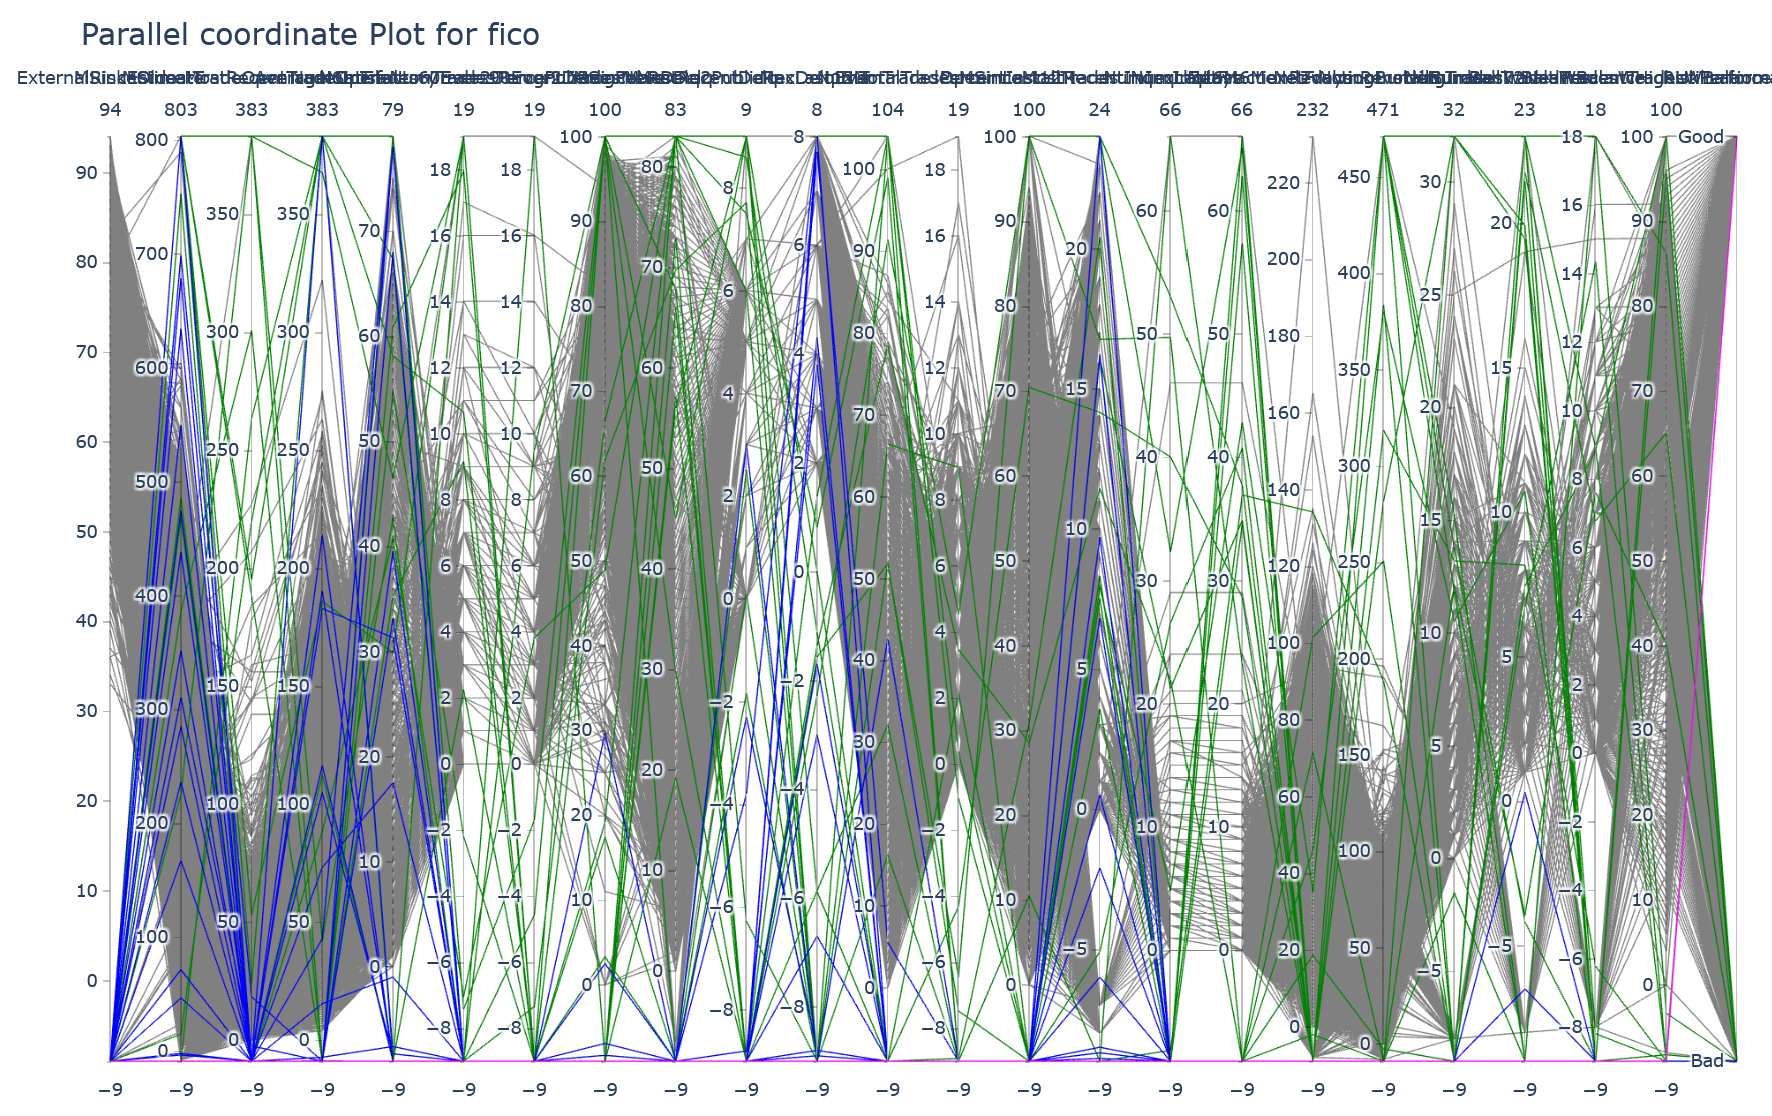
\includegraphics[width=\textwidth]{images/pcp-fico.png}
    \caption{Image of the parallel coordinates plot for the explainers on the fico dataset.}
    \label{fig:pcp-fico}
\end{figure}

What the above really suggests is that the counterfactual methods perform quite differently with between continuous and categorical features and that each method provides different kinds of counterfactuals. Given more time, the metrics could have also be measured separately for continuous and categorical features to find differences. Additionally, the metrics defined in section \ref{subsection:metrics} can be expanded since the Implausibility metric only measures the distances with respect to the nearest instance in the reference dataset. As a result, it does not respect the "concentration" of values within a dataset that can be seen in the parallel coordinates plots. To better represent realism, the following is the definition for this new metric:

% Mention Knn and KDE approach?
\textbf{Alignment}: Measures the Jaccard Index between the value ranges of counterfactuals and the instances in the same class as the counterfactuals. For continuous features, sample points that fall within the range are compared, and for categorical features, sets of unique values are compared. Higher values indicate better alignment. Let \(C\) denote the counterfactuals, \(T\) the CF target class instances:

For each continuous feature \( i \), let \(D_C^i\) be the subset of these points that lie within range (C), and \(D_T^i\)be the subset of points within range \(T\). Hence, the Jaccard index is calculated as:
\begin{equation}
J_{\text{cont}}^{i} =  \frac{|D_C^i \cap D_T^i|}{|D_C^i \cup D_T^i|}
\end{equation}

For each categorical feature \( j \), where \( C^j \) and \( T^j \) are the sets of unique categorical values for the counterfactuals and CF target class instances, the Jaccard index is given by:
\begin{equation}
J_{\text{cat}}^{j} = \frac{ | C^j \cap T^j | }{ | C^j \cup T^j | }
\end{equation}

The Alignment is the average of all individual feature alignment scores:
\begin{equation}
\text{Alignment} = \frac{1}{m_{\text{con}} + m_{\text{cat}}} \left( \sum_{i=1}^{m_{\text{con}}} J_{\text{cont}}^i + \sum_{j=1}^{m_{\text{cat}}} J_{\text{cat}}^j \right)
\end{equation}

The statistics corroborate the visual analysis. AIDE significantly outperforms DiCE and DiCE-genetic. The scores are also plotted for every dataset.

\begin{table}[!htbp]
    \centering
    \begin{tabular}{llrrrrl}
        \toprule
        Group 1       & Group 2         & Mean Diff & p-adj  & Lower     & Upper     & Reject \\
        \midrule
        AIDE          & DiCE-genetic   & -0.1327   & 0.0091 & -0.2379   & -0.0275   & True   \\
        AIDE          & DiCE  & -0.2186   & 0.0    & -0.3243   & -0.1129   & True   \\
        DiCE-genetic & DiCE  & -0.0859   & 0.1711 & -0.1984   &  0.0266   & False  \\
        \bottomrule
    \end{tabular}
    \caption{Table of Tukey's HSD Test results for Alignment (ANOVA p-value = \SI{8.0e-06}{})}
    \label{tab:tukey_alignment}
\end{table}

\begin{figure}[!htbp]
  \centering
  \begin{subfigure}{0.45\textwidth}
    \centering
    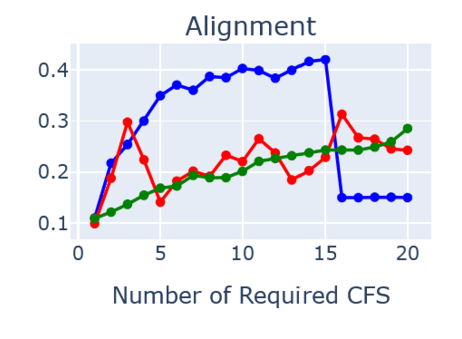
\includegraphics[width=\textwidth]{images/alignment-adult-1.png}
    \caption{adult dataset.}
    \label{fig:image1}
  \end{subfigure}
  \hfill
  \begin{subfigure}{0.45\textwidth}
    \centering
    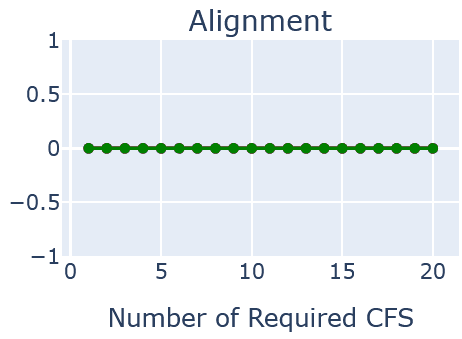
\includegraphics[width=\textwidth]{images/alignment-german_credit-1.png}
    \caption{german\_credit dataset.}
    \label{fig:image2}
  \end{subfigure}
  
  \vspace{0.5cm} 

  \begin{subfigure}{0.45\textwidth}
    \centering
    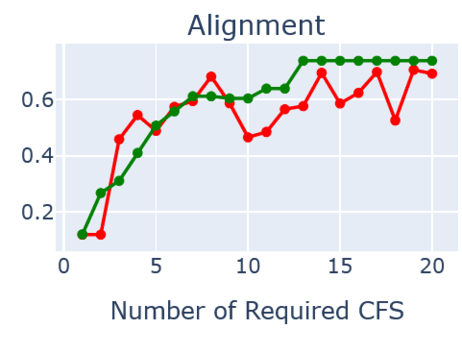
\includegraphics[width=\textwidth]{images/alignment-compas-1.png}
    \caption{compas dataset.}
    \label{fig:image3}
  \end{subfigure}
  \hfill
  \begin{subfigure}{0.45\textwidth}
    \centering
    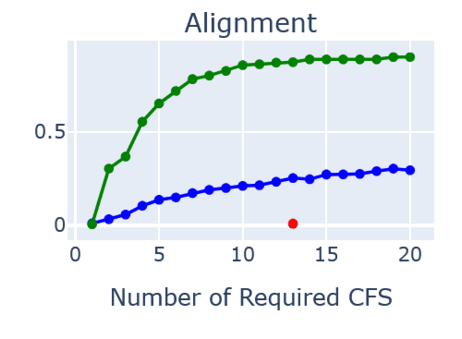
\includegraphics[width=\textwidth]{images/alignment-fico-1.png}
    \caption{fico dataset.}
    \label{fig:image4}
  \end{subfigure}
  
  \caption{Image of the Alignment metric for the explainers on the datasets, varying the required number of required counterfactuals. There seems to be the same issue as observed in Actionability with complex feature names in german\_credit.}
  \label{fig:four_image_grid}
\end{figure}